\documentclass{beamer}
\usetheme{Madrid}

\usepackage{amsmath, amssymb, amsthm}
\usepackage{graphicx}
\usepackage{listings}
\usepackage{gensymb}
\usepackage{minted}
\usemintedstyle{friendly}
\definecolor{bg}{rgb}{0.95,0.95,0.95}
\usepackage[utf8]{inputenc}
\usepackage{hyperref}
\usepackage{gvv}
\begin{document}
\title{NCERT 6.6.9}
\author{EE24BTECH11032 - JOHN BOBBY}
\date{}
\frame{\titlepage}
\begin{frame}{Question}
\textbf{Question:}A tank with rectangular base and rectangular sides, open at the top is to be constructed so that its depth is $2$ m and volume is $8$ $m^3$. If building of tank costs  $70$ per sq. meter for the base and  $45$ per square meter for sides. What is the cost of least expensive tank?\\
\end{frame}
\begin{frame}{Theoretical Approach}
\begin{align}
    Volume=\brak{2}\brak{x}\brak{y}=8\\
    xy=4\\
    \text{Total Cost}=70\brak{xy}+45\times2\brak{2x+2y}=280+180\brak{x+y}
\end{align}
From equation $\brak{2}$
\begin{align}
    \text{Total Cost}=280+180x+\frac{720}{x}
\end{align}
Differentiating wrt to x on both sides,
\begin{align}
    \frac{dy}{dx}=180-\frac{720}{x^2}
\end{align}
To be a critical point $\frac{dy}{dx}$  must be zero,
\begin{align}
    180-\frac{720}{x^2}=0\\
    x^2=\frac{720}{180},x=\pm 2\\
\end{align}

    
\end{frame}
\begin{frame}{}
  $x=2$, as length cant be negative\\
Checking $\frac{d^2y}{dx^2}$ to be positive for minimum
\begin{align}
    \frac{d^2y}{dx^2}=\frac{1440}{x^3}\\
    \frac{d^2y}{dx^2} >0\text{ for }  x=2
\end{align}
Thus $x=2$ is the minimum  
\end{frame}
\begin{frame}{Gradient Descent}
\begin{align}
    x_{n+1}=x_n-\alpha f^{\prime}\brak{x_n}\\
     x_{n+1}=x_n-\alpha \brak{180-\frac{720}{{x_n}^2}}
\end{align}
Where $\alpha$ is the learning rate,\\
This iteration will stop until we reach a stable state $\brak{f^{\prime}\brak{x} \approx0}$\\
We get,\\
$x_{min}=2$
\end{frame}
\begin{frame}[fragile]
\frametitle{C-Code}
\begin{minted}[bgcolor=bg, linenos, fontsize=\scriptsize, breaklines]{c}
#include <stdio.h>
#include <math.h>
void function(double *x,double *y,int n){
	for(int i=0;i<n;i++)
		y[i]=280+180*x[i]+720/(x[i]);
}
double derivative(double x){
	return 180-720/(x*x);
}
double  gradient_descent() {
    double l = 1.0;  // Initial guess for l (should be > 0 to avoid division by zero)
    double prev_l;
    do {
        prev_l = l;
        l = l - 0.001 * derivative(prev_l);
    } while (fabs(l - prev_l) > 1e-6);
    return l; 
}
\end{minted}
\end{frame}
\begin{frame}[fragile]
\frametitle{Python-Code}
\begin{minted}[bgcolor=bg, linenos, fontsize=\scriptsize, breaklines]{python}
import numpy as np
import matplotlib.pyplot as plt
import ctypes
import cvxpy as cp
# Load the shared library
lib = ctypes.CDLL('./lib.so')
lib.function.argtypes=[ctypes.POINTER(ctypes.c_double), ctypes.POINTER(ctypes.c_double), ctypes.c_int]
lib.derivative.argtypes=[ctypes.c_double]
lib.derivative.restype=ctypes.c_double
lib.gradient_descent.restype=ctypes.c_double
# Parameters
x_start = 0
x_end = 5
h = 0.01
n_steps = 501
# Setting up the array
x = np.linspace(x_start, x_end, n_steps)
y = np.zeros(n_steps)
# Conversion to ctypes array
x_ctypes = x.ctypes.data_as(ctypes.POINTER(ctypes.c_double))
y_ctypes = y.ctypes.data_as(ctypes.POINTER(ctypes.c_double))

\end{minted}
\end{frame}
\begin{frame}[fragile]
\begin{minted}[bgcolor=bg, linenos, fontsize=\scriptsize, breaklines]{python}
# Call the C functions
lib.function(x_ctypes, y_ctypes, n_steps)
min_point = lib.gradient_descent()
min_value = 280 + 180 * min_point + 720 / min_point
print(f"Minimum found at x = {min_point}, f(x) = {min_value}")
# Plotting
plt.figure(figsize=(10, 6))
plt.plot(x, y, label="Theory", linestyle='-', color='b', linewidth=5)
plt.scatter(min_point, min_value, color='r', marker='o', s=100, zorder=5, label=f"Min at x={min_point:.2f}")
plt.xlabel("x")
plt.ylabel("y")
plt.legend(['f(x)=280+180x+720/x', f'Min at x={min_point:.2f}'])
plt.grid()
plt.savefig('plot.png')
\end{minted}
\end{frame}
\begin{frame}[fragile]
\frametitle{CVXPY Module}
using Geometric Programming,
\begin{minted}[bgcolor=bg, linenos, fontsize=\scriptsize, breaklines]{python}
    #Define the variables
x=cp.Variable(pos=True)

#Define the objective function
objective=cp.Minimize(280+180*x+720/x)

#Defining the problem 
problem=cp.Problem(objective)

#Solving the problem with geometric programming
problem.solve(gp=True)
print("Results obtained from geometric programming")
print("Minimized x value: ",x.value)
print("Minimized cost value: ",problem.value)
\end{minted} 
\end{frame}
\begin{frame}{Plot}
\begin{figure}[h]
\centering
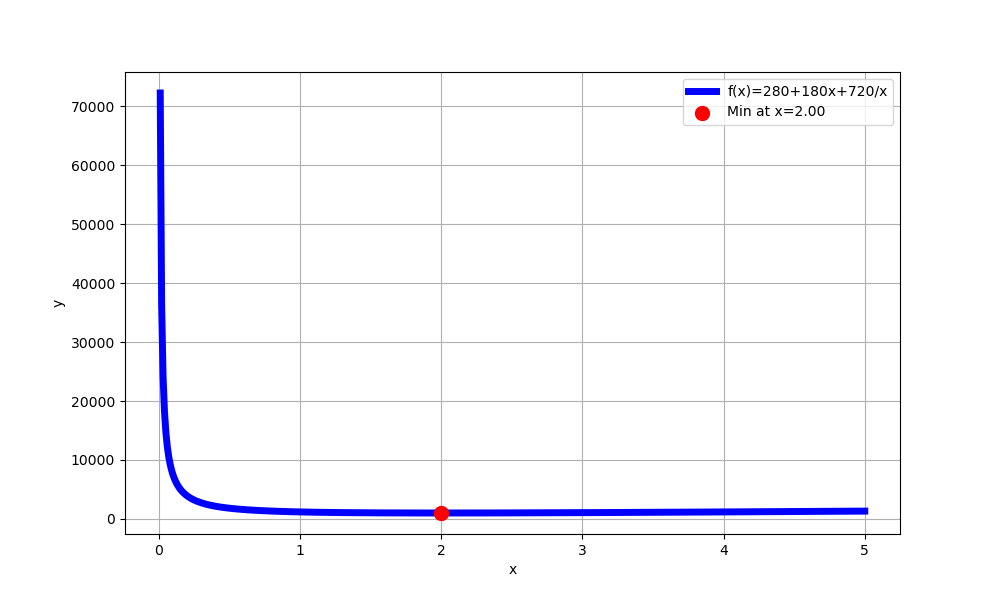
\includegraphics[width=\columnwidth]{figs/Q4.png}
\caption{Plot of the given question.}
\label{fig:Plot1} 
\end{figure}
    
\end{frame}



\end{document}
